\documentclass[a4paper,11pt]{style-esi/td}

\usepackage{style-esi/licence}	% Affiche une licence dans le document
\usepackage{style-esi/exercice}
\usepackage{style-esi/listing}
\usepackage{style-esi/tutoriel}
\usepackage{style/dev1}

\begin{document}

\seance{1}{NetBeans}{td01-introduction}{
	Dans ce TD vous ferez connaissance avec l'environnement intégré NetBeans et
	vous réaliserez vos premiers programmes en Java.
}

%===================
\section{NetBeans: environnement de développement intégré }
%====================	

\begin{Tutoriel}{Premier programme Java avec NetBeans}

	Vous allez être guidé pas à pas pour la création de votre tout premier programme Java.

	\begin{steps}
		\item Ouvrez NetBeans~:
		l'icône de l'application se trouve sur votre Bureau.

		\bigskip
		\begin{center}
			
\includegraphics{images/nb_icone}
		\end{center}

		%TODO: présentation générale de la fenêtre ?

		\item Créez un nouveau projet~:

		Pour cela, cliquez sur \og File \fg~en haut à gauche et ensuite, sur nouveau projet.

		\bigskip
		\begin{center}
			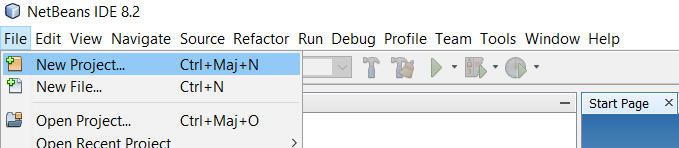
\includegraphics[width=.9\textwidth]{images/nb_newproject}
		\end{center}

		Dans la fenêtre \og New Project \fg~qui s'ouvre, choisissez \og Java Application \fg dans la liste \og Projects \fg~et cliquez le bouton \og Next \fg.

		A l'écran suivant \og New Java Application \fg~illustré ci-dessous,
		nommez le projet \texttt{td-java}, décochez la case \texttt{Create Main Class} et cliquez sur le bouton \og Finish \fg.

		\begin{center}
			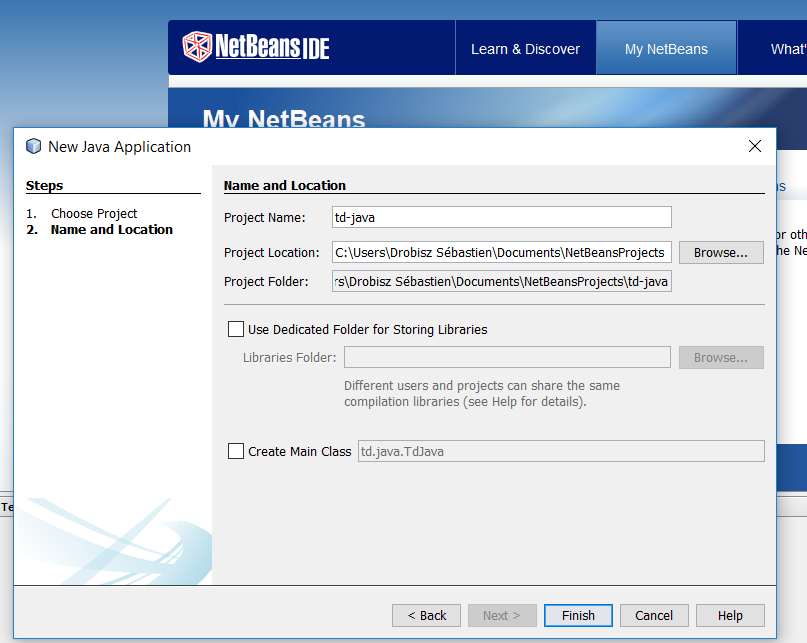
\includegraphics[width=.9\textwidth]{images/nb_newproject_name}
		\end{center}

		Dans NetBeans tout programme doit se trouver au sein d'un projet.
		Le projet contient le code de votre programme mais également les
		informations annexes comme le langage utilisé (ici Java),
		la version du langage (ici nous utilisons Java 8),
		et d'autres informations que vous découvrirez au fur et à mesure.

		% Un répertoire a été ajouté sur votre ordinateur. 	
		% Trouvez le et vérifiez le contenu du dossier contenant les sources de votre projet. 
		% Le dossier sur votre ordinateur s'appelle \texttt{src}. 
		% S'il est vide, c'est normal, vous n'avez pas encore ajouté de source.


		\item Créez un package~:

		faites un clic droit sur le dossier contenant les sources de votre projet
		(le code de votre programme), comme illustré dans l'image ci-dessous,
		et ajoutez un nouveau package Java.

		\bigskip
		\begin{center}
			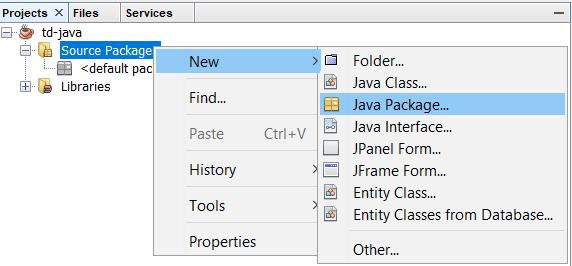
\includegraphics[width=.9\textwidth]{images/nb_newproject_package}
		\end{center}

		Nommez ce package \texttt{g12345.dev1.td1} où vous remplacez g12345 par votre identifiant et cliquez sur le bouton \og Finish\fg~:

		\bigskip
		\begin{center}
			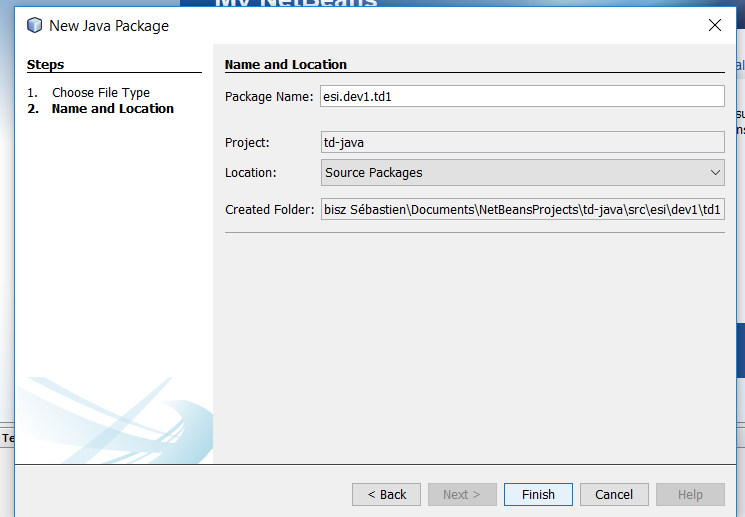
\includegraphics[width=.9\textwidth]{images/nb_newproject_package2}
		\end{center}

		En Java, un package (paquet) permet de regrouper certaines parties de votre code
		et ainsi d'ordonner votre projet.

		Remarquez que ce package a été ajouté dans les sources de votre projet.
		\bigskip
		\begin{center}
			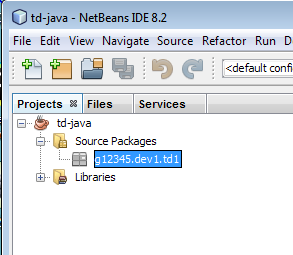
\includegraphics{images/nb_newproject_package3}
		\end{center}

		% Dans votre navigateur, vérifiez ce qui a été ajouté dans le dossier contenant vos sources.


		\item Créez une classe~:

		comme illustré sur l'image ci-dessous faites un clic droit sur votre package
		et ajoutez une nouvelle classe\footnote{Pour le moment,
			on va simplement dire que c'est un fichier dans lequel se trouve du code Java.}.
		Nommez cette classe {Hello}
		%\footnote{Si vous oubliez la majuscule au H, nous viendrons vous tirer les oreilles !}

		\bigskip

		\begin{center}
			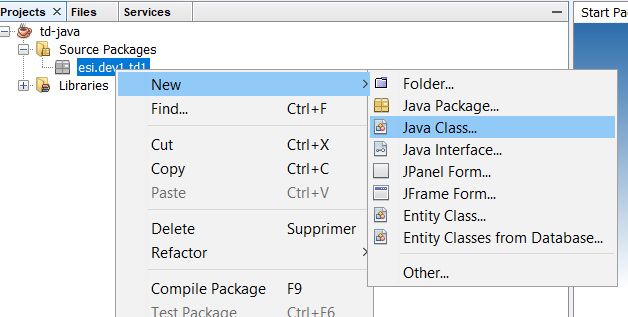
\includegraphics[width=.9\textwidth]{images/nb_newproject_new_class}
		\end{center}


		\item Ouvrez le fichier \texttt{Hello.java}~:

		double-cliquez sur votre classe \texttt{Hello}.
		Le code se trouvant dans ce fichier apparaît.

		%			%TODO: enlever le nettoyage ?
		%			Si vous voyez le code suivant, 
		%			veillez à l'effacer\footnote{Nous n'aimons pas le voir, il ne sert à rien}. 
		%			
		%			\begin{center}
		%				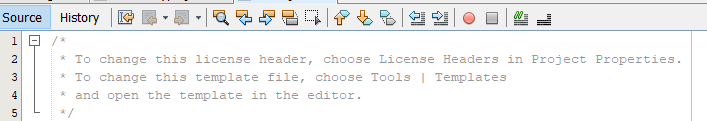
\includegraphics[width=\textwidth]{images/nb_newproject_header}
		%			\end{center}
		%			
		%			Faites la même chose pour le code contenant \texttt{/**...@author...*/}.

		Ajoutez le code suivant en respectant bien les
		minuscules et les majuscules~:

		\begin{Code}{java}
			public static void main(String[] args) {
					System.out.println("Hello, World!");
				}
		\end{Code}

		Vous devriez obtenir ceci :

		\begin{center}
			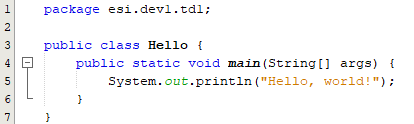
\includegraphics{images/nb_newproject_code}
		\end{center}
		Enregistrez vos modifications (control-s).

		\item Lancez le programme en cliquant sur la petite flèche \emph{run}

		
\includegraphics{images/nb_newproject_run}.

		Le résultat s'affiche dans la fenêtre intitulée \og Output \fg.
		Vous devriez voir "Hello, World !" s'y afficher.

		\item Créez un nouveau programme qui se nomme \texttt{"HelloPrénom"}. Celui-ci doit afficher \texttt{"Hello"} suivi de votre prénom.
		Si vous essayez de le faire tourner en cliquant sur la flèche, vous ne verrez pas apparaître votre prénom. C'est parce que Netbeans a retenu que le programme principal est le premier à avoir été lancé. Pour forcer Netbeans à lancer le nouveau programme, faite un clic droit sur le fichier \texttt{HelloPrénom.java} et cliquez sur \texttt{Run File}. Vous devriez voir "Hello, John" s'afficher dans l'output.

		\begin{center}
			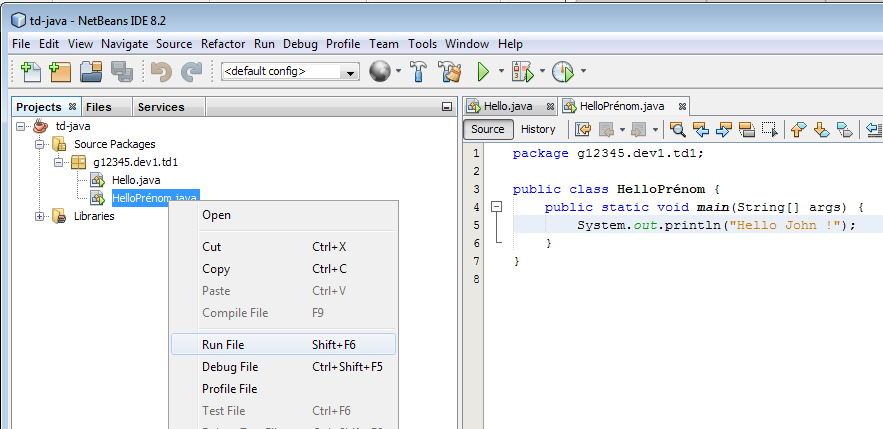
\includegraphics[width=.9\textwidth]{images/nb_newproject_run_othermain}
		\end{center}

	\end{steps}

\end{Tutoriel}

%===================
\section{Affichage}
%====================	

Le programme suivant affiche \texttt{Hello!} suivi de \texttt{Bonjour!}.
\listing{Java}{HelloBonjour.java}

\begin{itemize}
	\item La première ligne indique que la classe se trouve dans le package \texttt{esi.dev1.td1}
	\item La ligne 3 déclare la classe \texttt{HelloBonjour}, remarquez que le nom d'une classe
	      doit correspondre au nom du fichier dans lequel elle se trouve, ici \texttt{HelloBonjour.java}
	\item La ligne 5 déclare la \emph{méthode principale}, \emph{main} en anglais veut dire 'principale'.
	      C'est ici que commence votre programme.
	\item En java l'affichage se fait par l'\emph{instruction}: \texttt{System.out.println("Hello!");}
	\item Le texte entre guillemets sera affiché sur la \emph{sortie standard}, dans Netbeans la
	      sortie standard est la fenêtre "Output".
\end{itemize}

Le code source de la classe \texttt{HelloBonjour} (ainsi que tous les codes de ce TD) se trouvent à l'adresse~:

\url{\listingpublicpath}

Prenez l'habitude de copier dans votre projet Netbeans les codes présentés dans les TDs afin de
les exécuter sur votre machine.



%Exercices
\begin{Exercice}{Ligne}
	Dans votre package \texttt{g12345.dev1.td1} créez une classe \texttt{Exercice1}.
	Dans cette classe écrivez un programme  (et donc dans la méthode \texttt{main} de cette classe)
	qui affiche 10 tirets les uns à la suite des autres:

	\texttt{- - - - - - - - - -}
\end{Exercice}

\begin{Exercice}{Carré}
	Dans une classe \texttt{Exercice2} (dans votre package \texttt{g12345.dev1.td1}), écrivez un programme qui affiche un carré d'étoiles de 5 de côté:

	\begin{verbatim}
		*****
		*****
		*****
		*****
		*****
		\end{verbatim}
\end{Exercice}

\begin{Exercice}{Pyramide}
	Dans une classe \texttt{Exercice3}, écrivez un programme qui affiche une pyramide d'étoiles comme ceci:

	\begin{verbatim}
		   *
		  ***
		 *****
		*******
		\end{verbatim}
\end{Exercice}



%===================
\section{Expressions}
%====================	

Le programme suivant affiche la somme des \emph{nombres entiers}  12345678 et 87654321.

\listing{Java}{Expression.java}

\begin{itemize}
	\item	L'instruction de la ligne 6 affiche le texte entre guillemets~: \texttt{12345678+87654321 = }

	\item L'instruction de la ligne 7 affiche le \emph{résultat du calcul}
	      c'est-à-dire la somme de 12345678 et de 87654321~:  \texttt{99999999}

	\item Notez que l'\emph{expresssion} \texttt{12345678 + 87654321}
	      de l'instruction de la ligne 7 ne se trouve \emph{pas} entre guillemets.
\end{itemize}

Le nombre 12345678 est un nombre entier. Les nombres décimaux, aussi appelés flottants ou nombres à virgule, s'écrivent avec un point, par exemple: 12.3


\begin{Exercice}{Petits calculs}
	Dans une classe \texttt{Exercice4}, écrivez un programme qui affiche les expressions suivantes (sans effectuer le calcul) puis, à la ligne suivante,
	la valeur de l'expression, pour les expressions	suivantes:
	\begin{itemize}
		\item \texttt{10 + 32}
		\item \texttt{10 - 32}
		\item \texttt{2 * 21}
		\item \texttt{234 \% 57}
		\item \texttt{((2*2)+(3*3)) / 25}
		\item \texttt{12.3 + 13.5}
		\item \texttt{12.3 - 13.5}
		\item \texttt{12.3 * 13.5}
		\item \texttt{2.0 / 3.0}
	\end{itemize}

	Remarque: \texttt{\%} est l'opérateur modulo c'est-à-dire le reste de la division entière.
	\texttt{/} est l'opérateur de division ici division entière. Par exemple,
	\texttt{37\%10} vaut 7 et \texttt{37/10} vaut 3.

\end{Exercice}

\begin{Exercice}{Divisions entière et décimale}
	Dans une classe Exercice5, créez un programme qui affiche, de même, les
	expressions à évaluer puis leur valeur pour les expressions suivantes:

	\begin{itemize}
		\item \texttt{2.0 / 3.0}
		\item \texttt{2 / 3}
		\item \texttt{2 / 3.0}
		\item \texttt{2.0 / 3}
		\item \texttt{2.0 / 0.0}
		\item \texttt{2 / 0}
	\end{itemize}

	Notez la différence de résultat entre les expressions \texttt{2.0/3.0} qui est une division entre nombres décimaux
	et \texttt{2/3} qui est une division entre entiers (et donc une division entière).

	Notez également la différence de résultat entre les 2 dernières expressions qui sont des divisions par zéro.
	La première est une division entre nombres décimaux,
	la seconde est une division entre entiers.
\end{Exercice}
%	\newpage
%	\begin{Exercice}{Felix}
%		\'Ecrivez un programme qui affiche le dessin suivant:
%
%	\begin{verbatim}
%	                          :                      :M
%	                         XMX                   .HMM>
%	                         MMMM.                dMMMM>
%	                        'MMMMMX     .....   dMMMMMMX
%	                        XMMMMMMMnMMMMMMMMMMMMMMMMMMM
%	                       :MMMMMMMMMMMMMMMMMMMMMMMMMMMM>
%	                       XMMMMM!"    "MMMMMM"`  `"MMMMM
%	                       MMMM#         4MMf        `MMMX
%	                      XMMM            MX          'MMM:
%	                     'MMM~            '>            MMM
%	                     MMMf       .     '>            `MMX
%	                    MMMM>     :MMM    '>   :MMM      MMMX
%	                   XMMMM      MMMM>   '>   XMMMX     MMMMk
%	                  MMMMMM>     MMMM~   'k   MMMMX     MMMMMh
%	                 MMMMMMMX     XMMM    XX   ?MMM     XMMMMMMM
%	                 MMMMMMMMk     ^`    X 'h    `     :MM##MMM~
%	                  ?MM>  ^?M.       .!    %.      .HM"   MM
%	                 .?M      '"%+++!".nMMMMn "%++!*" %.. 'M..
%	                  `?M>+%L         <MMMMMMMM>       :   XM"
%	                    'X   %        XMMMMMMMM>      X   'f
%	                      X   `M.      ?MMMMMM~    .HM   :`
%	                       %.  `MMMx.          .xHMMM   X
%	                  ..    `X  `MMMMMMMMMMMMMMMMMMM  :f
%	                :MMMMMMMh:.M. 4MM     "     MM" xMMMMMMMMMMh.
%	              :MMMMMMMMMMMMMMM: `%x.......x"`.HMMMMMMMMMMMMMM
%	            .MMMMMMMMMMMMMMMMMMMMhx.......xHMMMMMMMMMMMMMMMMM
%	    .nHMMMMMMMMMMMMMMMMMMMMMMMMMMMMMMMMMMMM`MMMMMMMMMMMMMMMMX
%	  :MMMMMMMMMMMMMMMMMMMMMMMMMMMMMMMMMMMMdMMMMMMMMMMMMMMMMMMMM
%	 MMMMMMMMMMMMMMMMMMMM"``""MMMMMMMMMMMM!MMMMMMMMMMMMMMMMMMMM~
%	MMMMMMMMMMMMMMMMMMM!     XMMMMMMMMMMMf:HMMMMMMMMMMMMMMMMM!
%	M?MMMMMMMMMMMMMMMM`    :MMMMMMMMMMMM!MMMMMMMMMMMMMMMMMMM~
%	:MMMMMMMMMMMMMMMMX     MMMMMMMMMMMMXXMMMMMMMMMMMMMMMMM`
%	MMMMMMMMMMMMMMMMMX    'MMMMMMMMMMMMM!MMMMMMMMMMMMMMMMX
%	MMMMMMMMMMMMMMMMM~    'MMMMMMMMMMMMMM?MMMMMMMMMMMMMMM~
%	 #M)MMMMMMMM!MMM       MMMMMMMMMMMMMMMM/MMMMMMMMMMMM~
%	   ?MMMMMM"-"2MMMMMx   XMMMMMMMMMMMMMMMMX?**!:MMM"`
%	\end{verbatim}
%\end{Exercice}




\end{document}
